%!TEX root = ../dokumentation.tex

\section{Content Modeling}

\subsection{Iterationsstufe 1}
\subsubsection{Abstract Prototype 1}

User environment design Schaffen eines Architekturmodells, das zeigt, wie die einzelnen Systemkomponenten zusammen in Beziehung stehen. Repräsentieren der Struktur- und der Funktions- Cluster des Systems unabhängig von Aspekten des Benutzerinterfaces 
oder der Implementierung

Sicherstellen, dass der Arbeitsfluss innerhalb des Systems die Arbeit unterstützt wird. Unterstützen der Designer in der Konzentration auf Arbeitsfluss und Funktion in dem System anstelle der Betrachtung von Benutzer Interface und Implementierung. Schaffen von System-Repräsentationen, die Planung unterstützen

 Abstract Prototyping\\
 content of user interface ohne zu zeigen wie es aussieht\\

 Content Modeling \\
 inhalte des user interface ohne details zum aussehen
 content model = sammlung von material (was den user interessiert zu sehen oder zu ändern), tools (ermöglichen den user dies zu tun) und working spaces(teile die tools und materials verbinden)\\

 Papier = working spaces (post it = tools and materials)
 content model + navigation map

 conceptual scenarios£


Hartmann S442
Abb. \ref{interfaceContents1}

\begin{figure}[H]
\centering
\hfill
\subfloat[aktionAuswählen \label{pic:aktionAuswaehlen}]{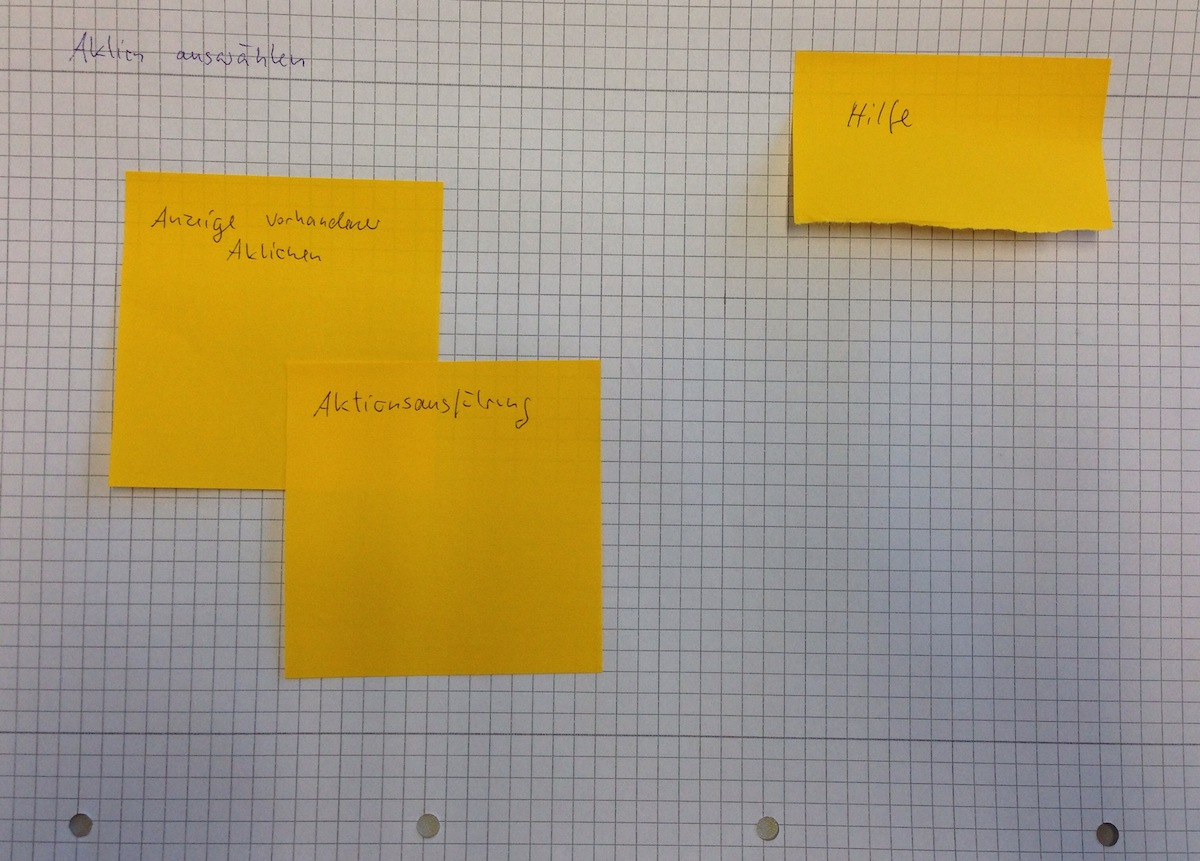
\includegraphics[width=.5\textwidth]{./images/abstract/version1/aktionAuswaehlen.JPG}}
\hfill % alternativ auch \hspace{1cm} für genaue Angaben
\subfloat[sucheMietobjekt \label{pic:sucheMietobjekt}]{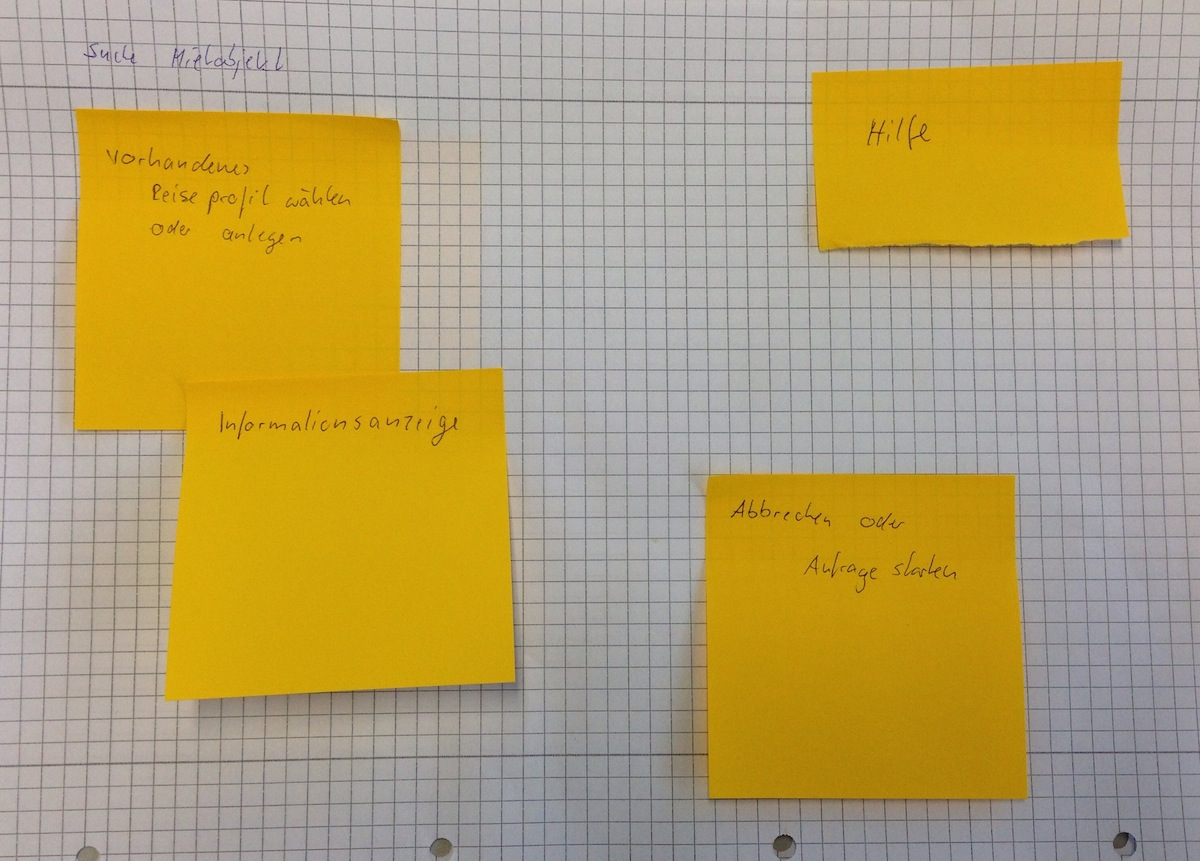
\includegraphics[width=.5\textwidth]{./images/abstract/version1/sucheMietobjekt.JPG}}
\hfill %
\caption{Inter. Context AP1: aktionAuswählen und sucheMietobjekt }
\label{interfaceContents1}
\end{figure}

Abb. \ref{fig:navigationmap1}
\begin{figure}[H]
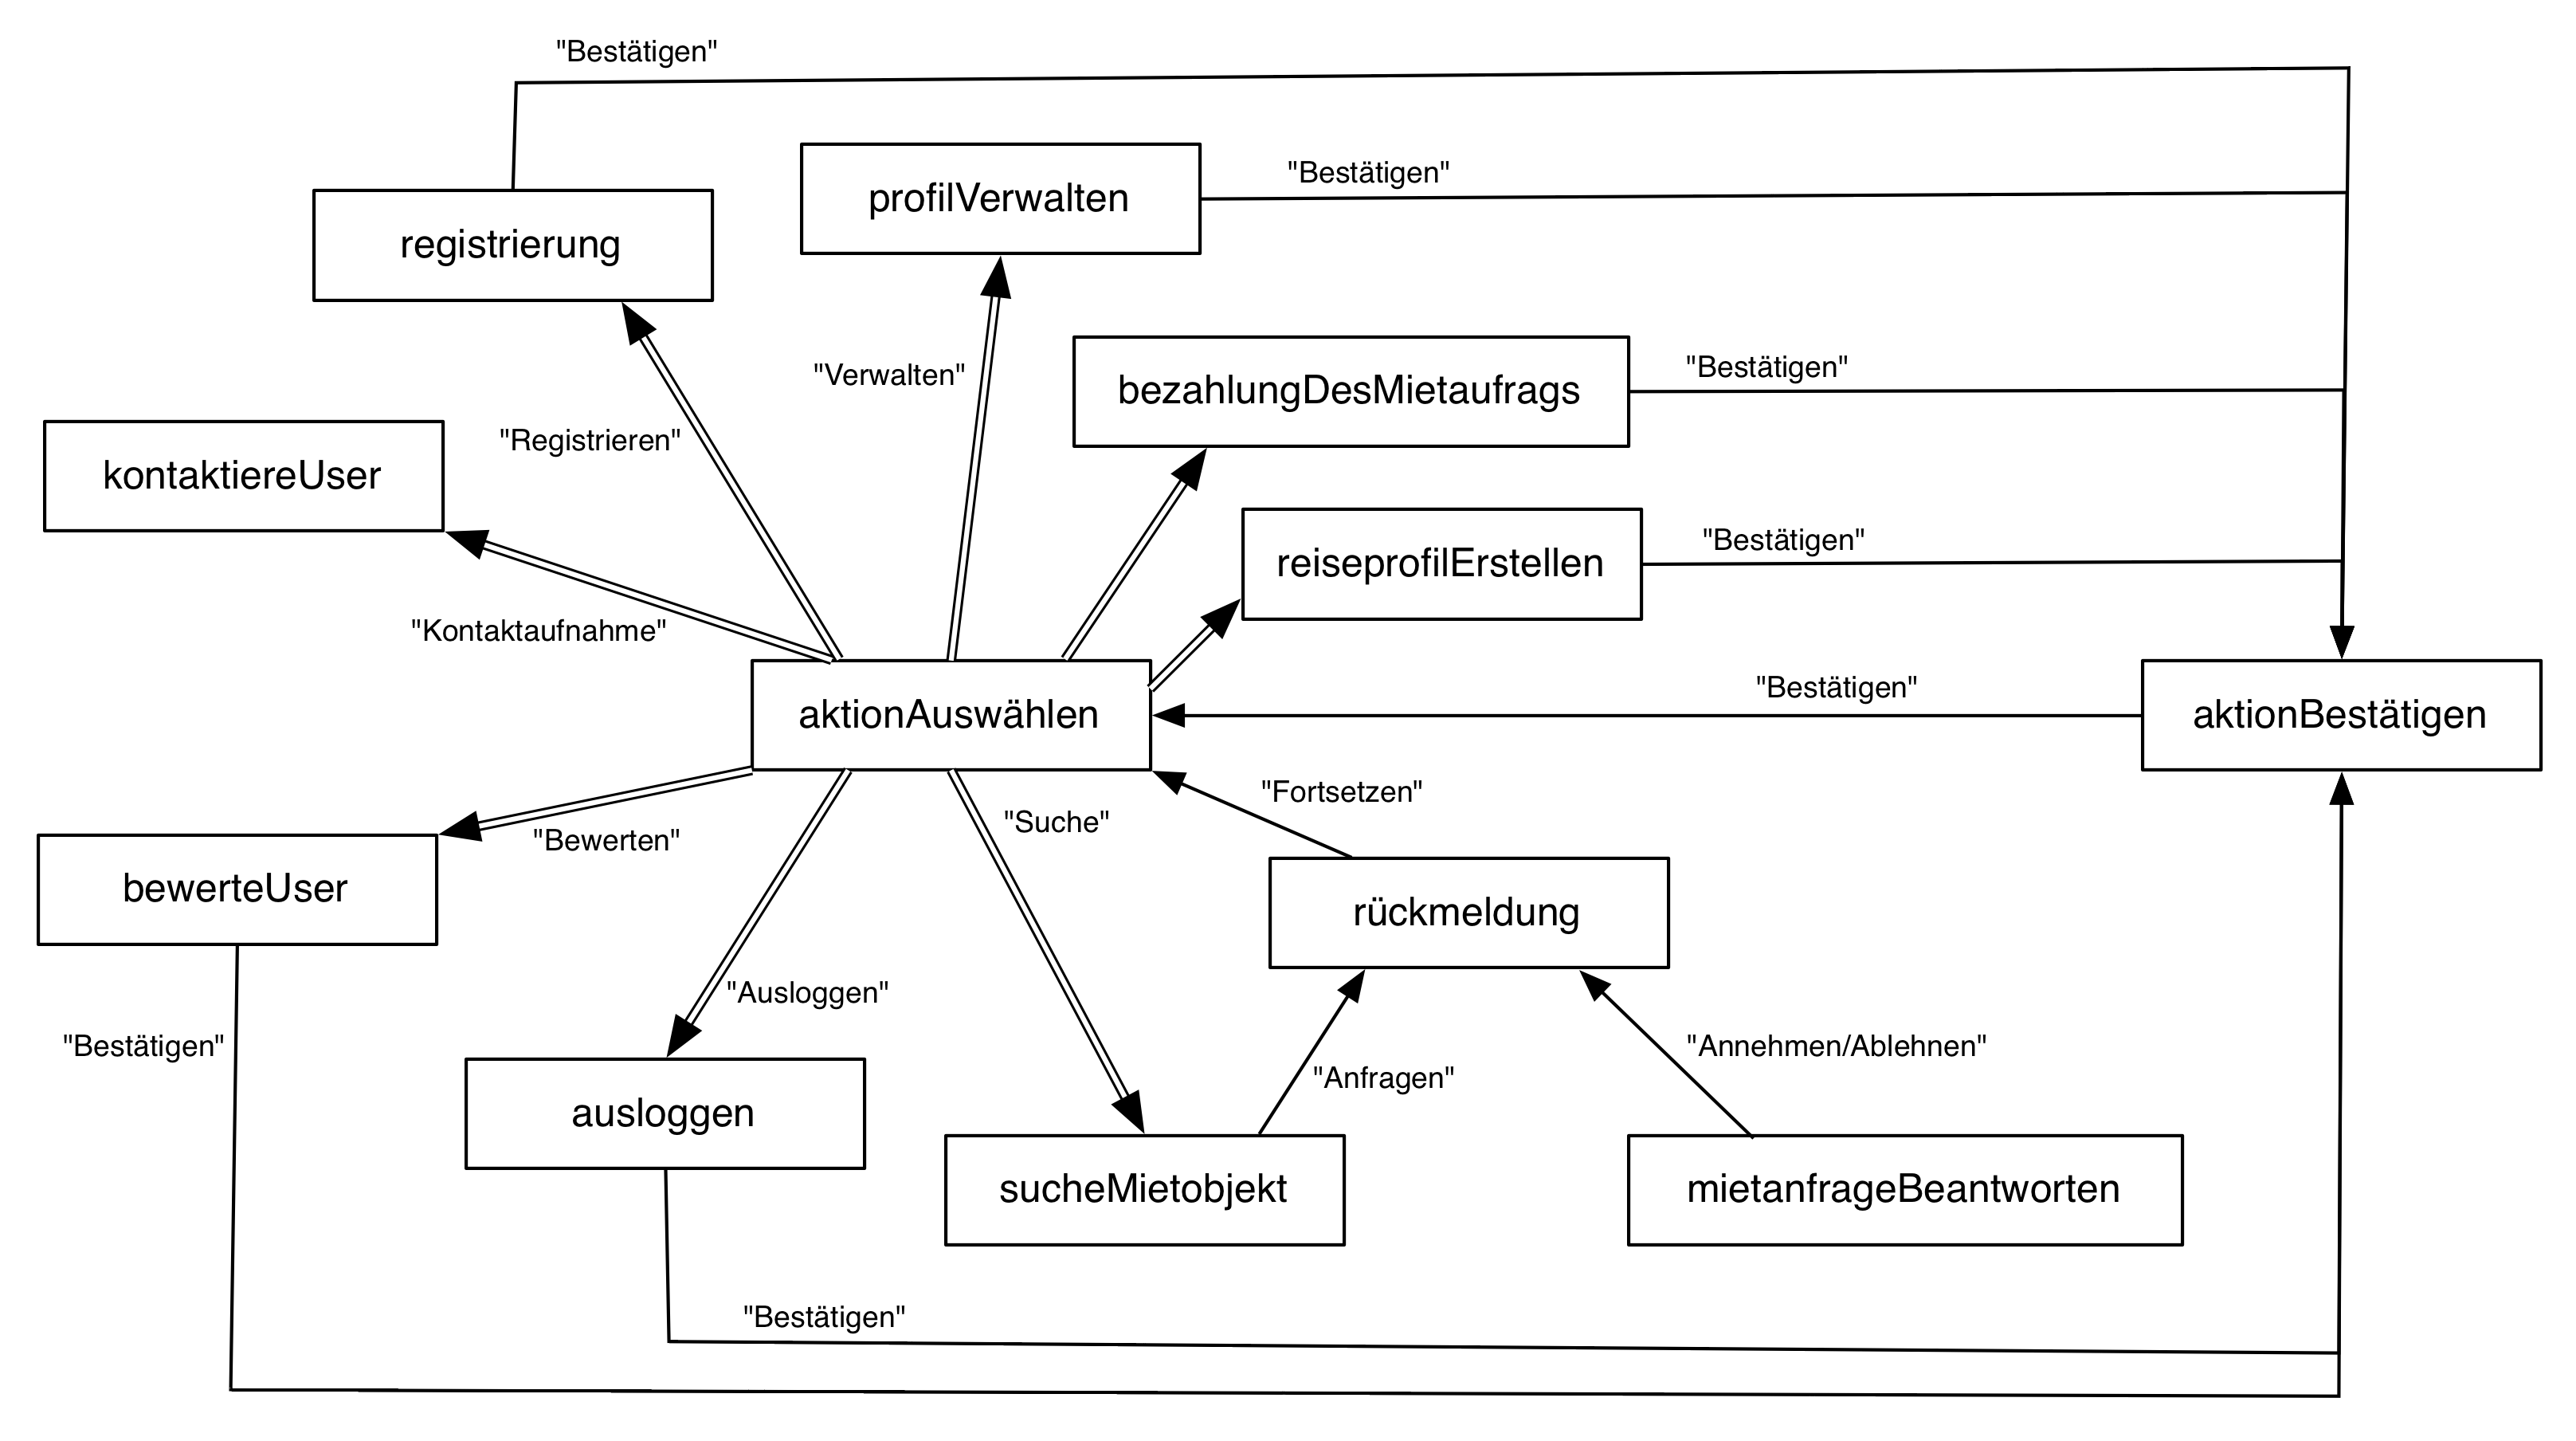
\includegraphics[width=1\textwidth]{./images/navigationmap1.png}
\caption{Context Navigation Map Version 1}
\label{fig:navigationmap1}
\end{figure}


\newpage
\subsubsection{Evaluation}

\subsection{Iterationsstufe 2}
\subsubsection{Abstract Prototype 2}


Abb. \ref{interfaceContents2}

\begin{figure}[H]
\centering
\hfill
\subfloat[anzeigenVorhandenerAktionen \label{pic:anzeigenVorhandenerAktionen}]{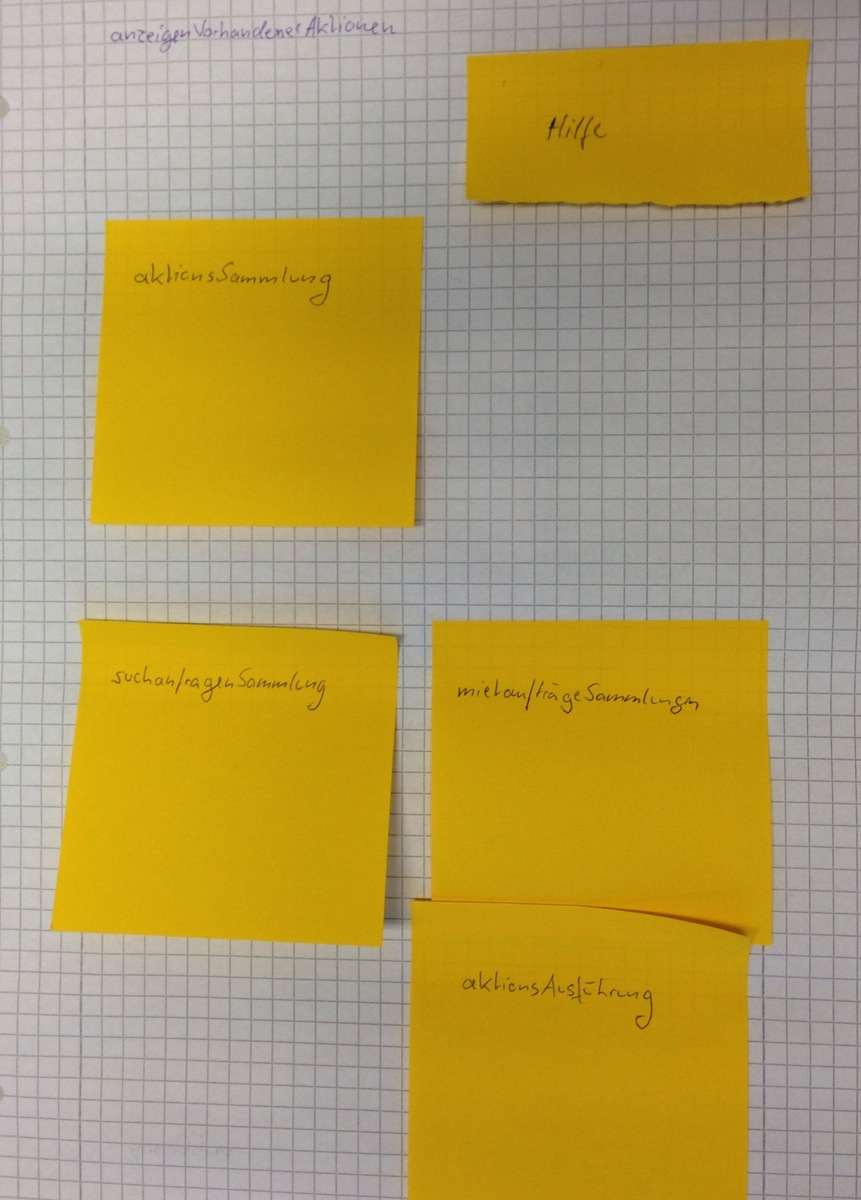
\includegraphics[width=.5\textwidth]{./images/abstract/version2/anzeigenVorhandenerAktionen.JPG}}
\hfill % alternativ auch \hspace{1cm} für genaue Angaben
\subfloat[suchanfrageStarten \label{pic:suchanfrageStarten}]{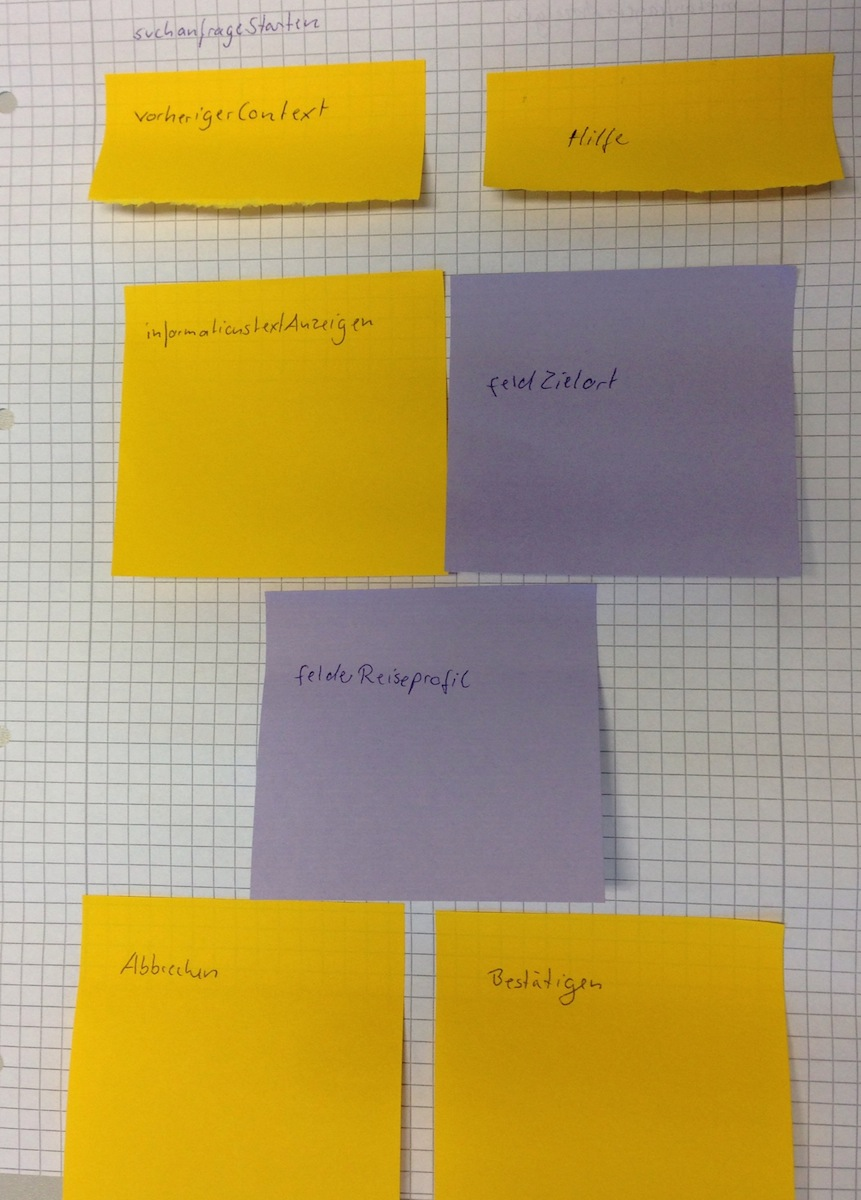
\includegraphics[width=.5\textwidth]{./images/abstract/version2/suchanfragenStarten.JPG}}
\hfill %
\caption{Inter. Context AP2: anzeigenVorhandenerAktionen und suchanfrageStarten }
\label{interfaceContents2}
\end{figure}

testestsetset

Abb. \ref{fig:navigationmap2}
\begin{figure}[H]
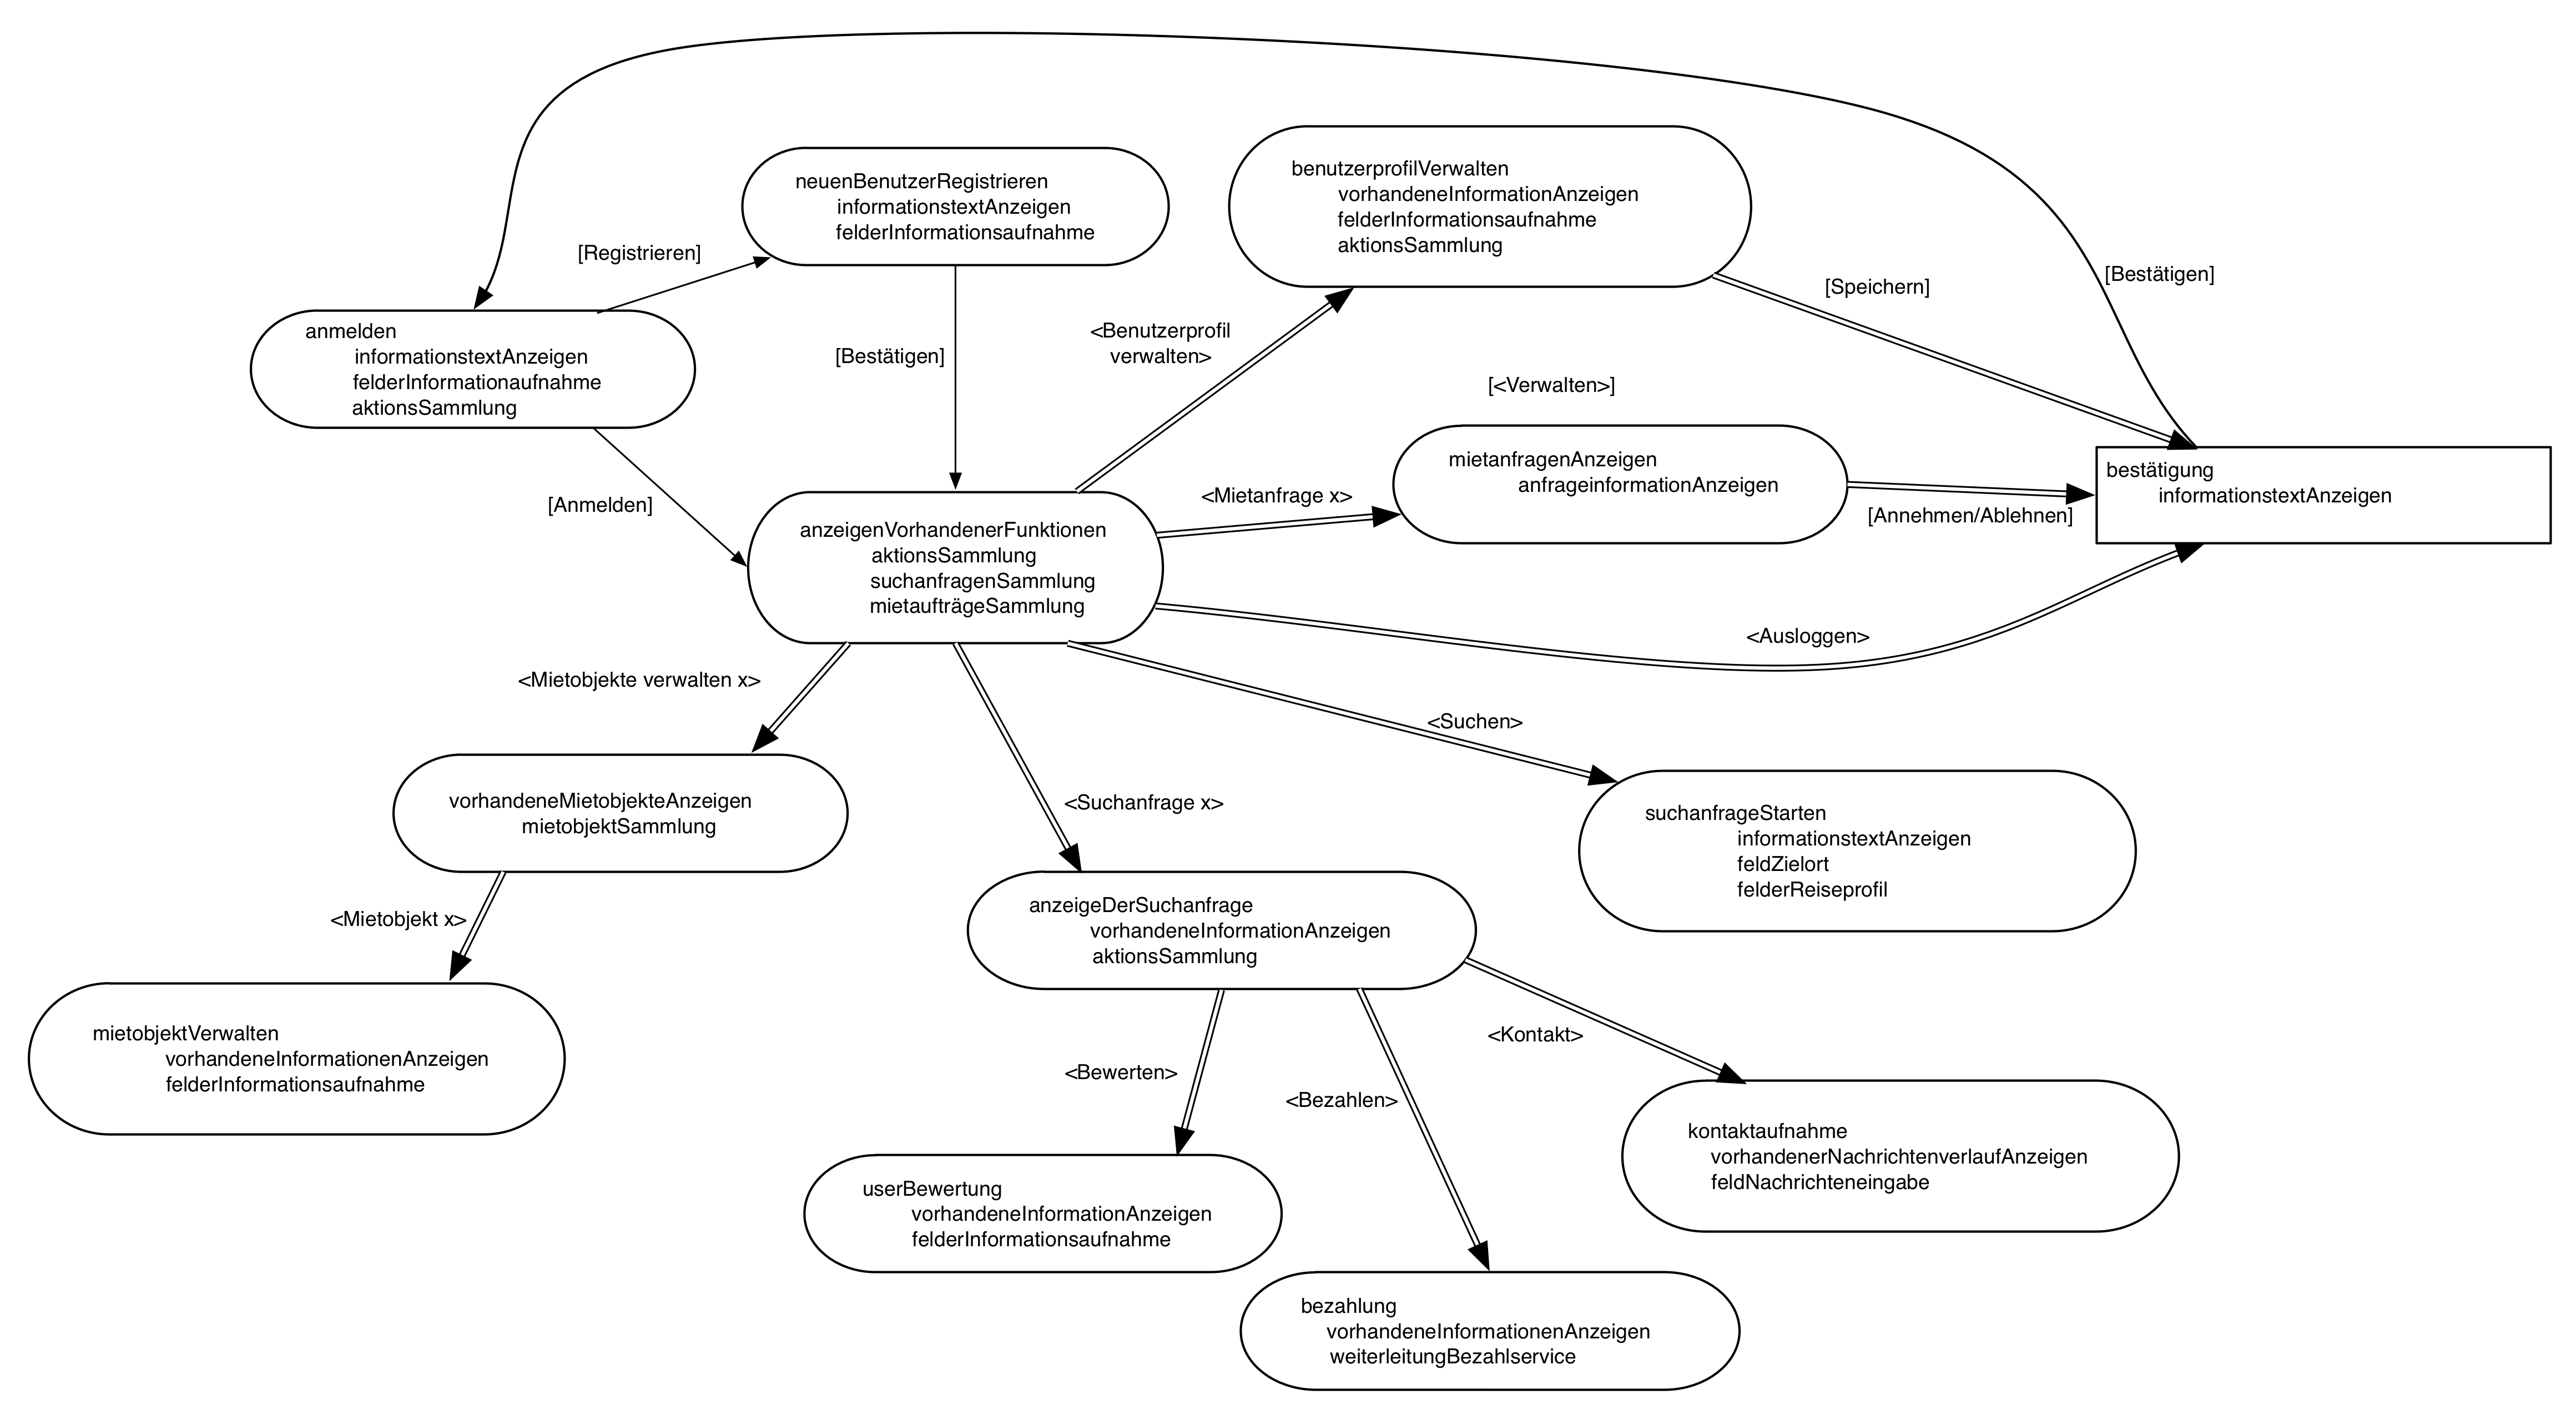
\includegraphics[width=1\textwidth]{./images/navigationmap2.png}
\caption{Context Navigation Map Version 2}
\label{fig:navigationmap2}
\end{figure}


